\documentclass[a4paper,10pt]{article}
\usepackage[english]{babel}
\usepackage[utf8]{inputenc}
\usepackage{url}
\usepackage[margin=1in]{geometry}
\usepackage{enumitem}

\usepackage[nottoc]{tocbibind}
\usepackage{fancyvrb} 
\usepackage{float}
\usepackage{graphicx}
\usepackage{subcaption}
\usepackage{color}
\usepackage{booktabs}
\usepackage{listings}

\title{Combinatorial Optimization\\Homework 4 – Genetic Algorithm}
\author{Matyáš Skalický\\skalimat@fit.cvut.cz}

\begin{document}
\maketitle
\tableofcontents
\medskip

\section{Experiment Setting}
In this homework, we are solving the bound knapsack problem by using a black-box solver - genetic algorithm. We are using the instances of size 40 from the pre-calculated \emph{NK40} dataset.

To make the measurements fair across different population sizes (also further called batch), each experiment was ran for \emph{3 seconds} of the CPU time and the best found solution for each bag was recorded.

\section{Genetic Algorithm}

The implemented genetic algorithm solver is parametrized mainly by 2 hyperparameters - the \emph{mutation rate} and \emph{batch size}. Batch size controls the size of the population.

Generally speaking, we first spawn a pool of instances created by the random initialization strategy (described below). Then before the time runs out, we repeatedly take a batch of parent instances, and by using selection, recombination and mutation, we create a pool of children of the same size. The detailed steps are described below.

\subsection{Fitness}

Fitness is defined as the total cost of items in the bag. If the bag's weight crosses the capacity, the fitness is set to $0$ regardless the value of the bag.

\subsection{Random Initialization}

I've implemented 2 initialization strategies for instance intialization. The \emph{naive} strategy simply selects one item in the bag randomly. So each new bag contains just 1 randomly selected item. The \emph{random} strategy is somewhat more sophisticated as it tries to add items into the bag in a random order until the capacity is reached. This strategy will thus produce bags, that are less sparse.

\subsection{Selection}

Selection takes a pool (batch) of candidates on the input. It calculates the total fitness and uses the roulette wheel selection to find the pairs of candidates that go into recombination.

\subsection{Recombination}

We take 2 input instances ('parents'). A single-point crossover is used to create 2 children. If any of the children is valid (fitness is non-0), we return the better child. Otherwise, the better parent is returned.

\subsection{Mutation}

Mutation is controlled by the \emph{mutation\_rate} hyperparameter. It is called on the instances that come out of recombination before we add them into children pool We randomly flip the indicator (whether the thing is, or is not in the bag) with the probability defined by the \emph{mutation\_rate}.


\section{Experiments}

As described above, we are running each experiment for 3 seconds of the CPU time to make different batch sizes comparable (small batches will be much faster, but there will be less diversity in the population).

\subsection{Pilot Experiments}

During the pilot experiments, we would like to determine the ideal mutation rate and batch size to solve the bag problem of instance size 40. We will also try to see, whether there is a notable difference between the random initialization strategy and the naive initialization strategy (which will produce much more spares initial instances).

\begin{figure}[!htb]
	\centering
  	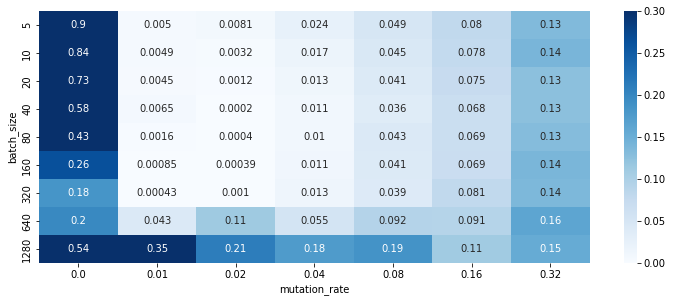
\includegraphics[width=\textwidth]{images/pilot_naive.png}
	\caption{Naive Initialization; NK40 Dataset; 3s Runtime; 100 Instances Mean Relative Error}
	\label{pilot_naive}
\end{figure}

As described before, the naive initialization produces very sparse bags. With very low mutation rate, there isn't enough diversity in the initial population pool to achieve good performance. As we can see in the Figure \ref{pilot_naive}, a small mutation rate is required. Interesting finding is that we are able to solve the problem even with a very small batch size. Even though the batch size is very small, the algorithm will be very fast. And it is able to go through many iterations before the time runs out.

\begin{figure}[!htb]
	\centering
  	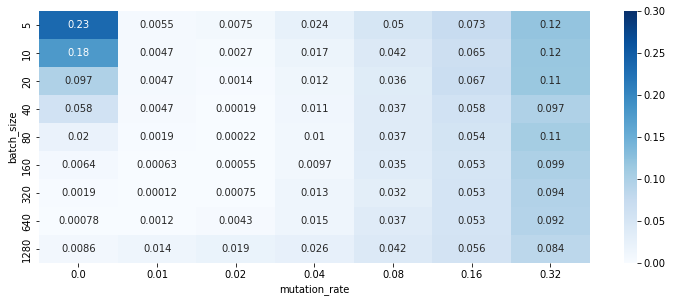
\includegraphics[width=\textwidth]{images/pilot_random.png}
	\caption{Random Initialization; NK40 Dataset; 3s Runtime; 100 Instances Mean Relative Error}
	\label{pilot_random}
\end{figure}

The random initialization contains fuller bags which contain a larger number of items. Figure \ref{pilot_random} shows, that even if the mutation rate is $0$, the algorithm achieves good results given large batch size. 

\subsection{Detailed Experiment}

The random initialization strategy has worked slightly better than the naive strategy. The best set of hyperarameters would be batch size of $320$ and mutation rate of $0.02$ (2\%). We will now look in a finer detail at the fitness score over time for the best obtained hyperparameter combination.

\begin{figure}[!htb]
	\centering
  	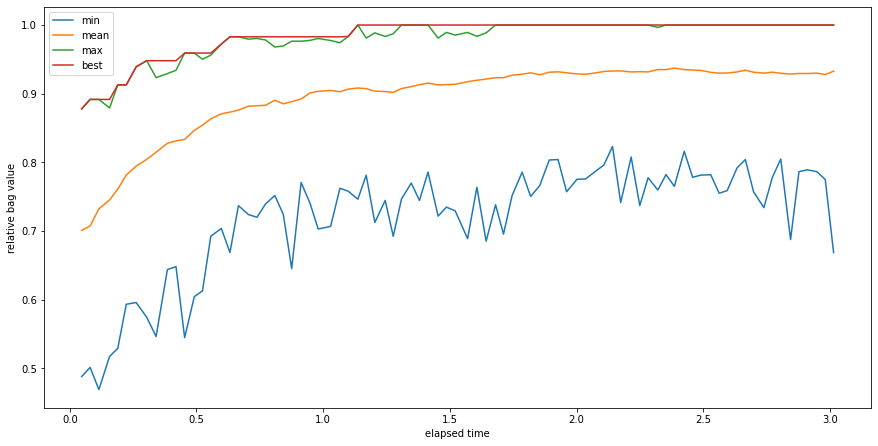
\includegraphics[width=\textwidth]{images/detail.png}
	\caption{Random Initialization; 3s Runtime; Instance Size 40}
	\label{detail}
\end{figure}

As we can see in the Figure \ref{detail}, for the instance above, the ideal solution was found just after $1$ second. Yet, we can see that the mean relative bag value across the population is still going up. It however levels after $2$ seconds.

\clearpage
\section{Discussion and Takeoffs}

Fourth homework was much more fun compared to the previous one. Genetic algorithms are one of my favorite black-box methods and even though I've implemented them several times, I still had fun applying it on the knapsack problem.

There was one interesting takeaway that came from the way I measured the experiment in the pilot phase (fixed amount of CPU time). The algorithm was able to find a good solution even with a very small population size of $5$ given that the mutation was turned on and was small. This is because the algorithm is able to go through a large amount of iterations before the time runs out as opposed to the large populations. But this relates to the NK algorithm and the knapsack problem itself.

\end{document}